\chapter{Opis projektnog zadatka}
		
		%\textbf{\textit{dio 1. revizije}}\\
		
		%\textit{Na osnovi projektnog zadatka detaljno opisati korisničke zahtjeve. Što jasnije opisati cilj projektnog zadatka, razraditi problematiku zadatka, dodati nove aspekte problema i potencijalnih rješenja. Očekuje se minimalno 3, a poželjno 4-5 stranica opisa.	Teme koje treba dodatno razraditi u ovom poglavlju su:}
		%\begin{packed_item}
			%\item \textit{potencijalna korist ovog projekta}
			%\item \textit{postojeća slična rješenja (istražiti i ukratko opisati razlike u odnosu na zadani zadatak). Dodajte slike koja predočavaju slična rješenja.} %dodaj slike %
			%\item \textit{skup korisnika koji bi mogao biti zainteresiran za ostvareno rješenje.}
			%\item \textit{mogućnost prilagodbe rješenja } 
			%\item \textit{opseg projektnog zadatka}
			%\item \textit{moguće nadogradnje projektnog zadatka}
		%\end{packed_item}
		
		%\textit{Za pomoć pogledati reference navedene u poglavlju „Popis literature“, a po potrebi konzultirati sadržaj na internetu koji nudi dobre smjernice u tom pogledu.}
		 \text Naš cilj jest napraviti web aplikaciju, Autos, za iznajmljivanje vozila privatnim i poslovnim korisnicima. \par 
		 \text Cilj projekta upoznavanje je i praktična primjena postupaka oblikovanja programske podrške sa zadaćama ostvarenja zahtjeva ovog zadatka, shvaćanje važnosti i značenja projektne dokumentacije i stvaranje spomenute dokumentacije. Važna je i što preciznija implementacija zahtjeva i poboljšanje vještina u svim područjima potrebnim za uspješno implementiranje zadatka. Uz programiranje i rad dokumentacije, jedna od vrijednih vještina koje ćemo steći jest znanje o raspodjeli rada i iskustvo suradnje s timom ljudi u svrhu ostvarenja zajedničkog projekta. \par 
		 \text U poslovanju vezanim uz iznajmljivanje automobila već postoji znatan broj poduzeća koje nude sličan model onom koji mi nastojimo ostvariti. Priložen je jedan primjer. \par 
		 
		 \begin{figure}[hp]
                \centering
                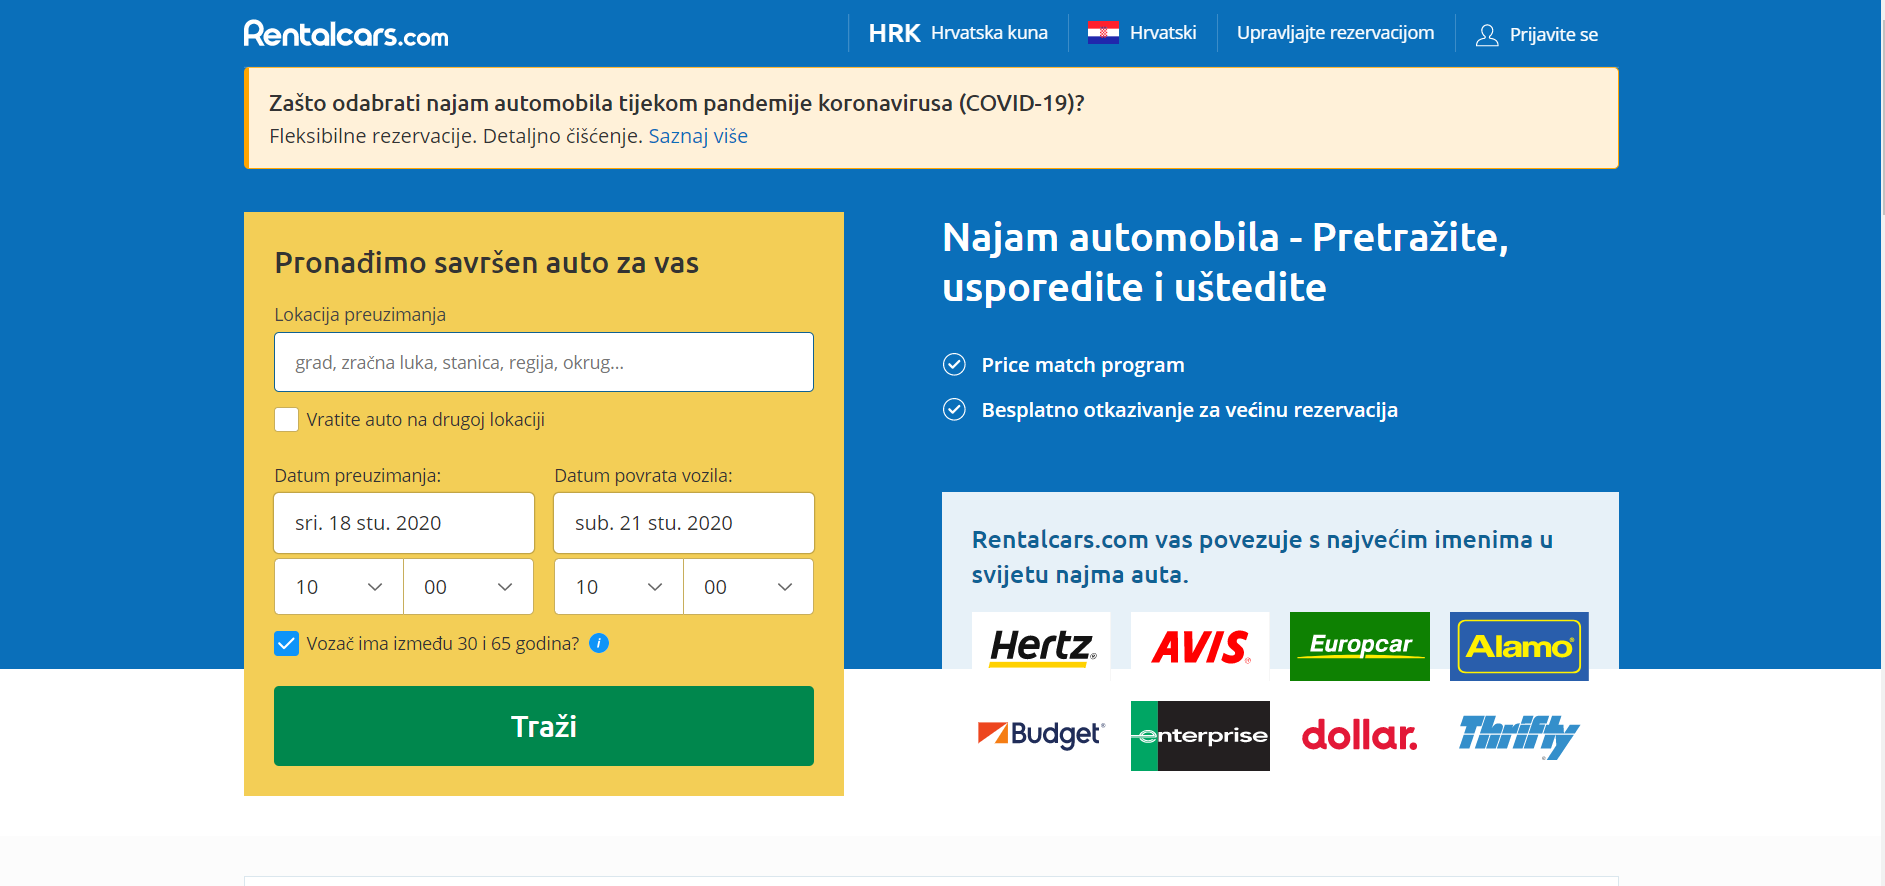
\includegraphics[width=15cm]{slike/stranica1.png}
                \caption{\textit{Izvor: rentalcars.com}}
            \end{figure}

		 \text Kao što vidimo u primjeru nudi se datum i vrijeme preuzimanja te datum i vrijeme vraćanja vozila te lokacija preuzimanja i lokacija vraćanja vozila. U web aplikaciju omogućena je prijava i odabir načina plaćanja. \par 
		%\text
		\pagebreak
		 
		 \begin{figure}[h]
                \centering
                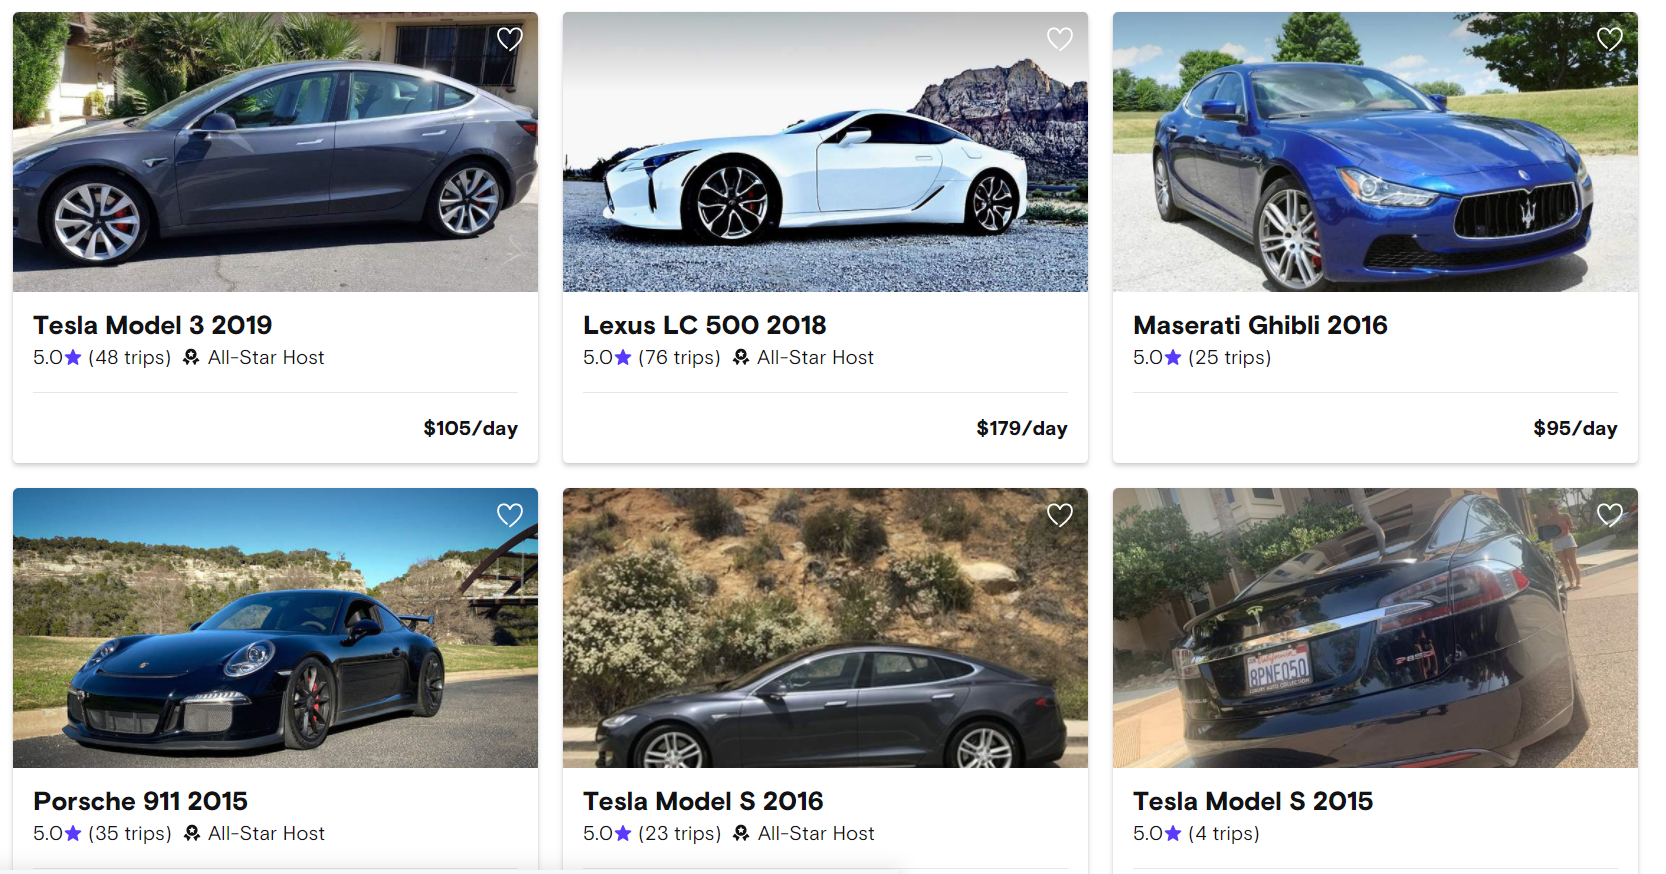
\includegraphics[width=15cm]{slike/stranica2.png}
                \caption{\textit{Izvor: turo.com}}
            \end{figure}
            
		 \text U primjeru iznad vidljiv je i izbor pojedinog automobila za iznajmljivanje. \par

		 
		 \text Godišnje oko 580 milijuna ljudi u svijetu koristi usluge iznajmljivanja vozila, a 70 posto tih ljudi iznajmi vozilo preko interneta. Ukupan broj korisnika ovih usluga kao i postotak njih koji usluge koristi preko interneta u porastu je i nastavak tog porasta očekuje se kroz sljedećih nekoliko godina. \par
		 \text Jedan od zahtjeva zadatka jest stvoriti mogućnost prijave i registracije korisnika za koju je potrebno unijeti ime, prezime i adresu elektroničke pošte. \par 
         \text Implementacija će sadržavati četiri različite vrste korisnika: administrator, vlasnik sustava,
korisnik (najmoprimac vozila) i neprijavljeni korisnik (gost). \par
        \text Administrator upisuje sve podatke o poduzeću (kao što su nove poslovnice) i definira tko ima ulogu vlasnika. Može vidjeti koji su trenutno aktivni korisnici i njihov ukupan broj.\par 
\text Vlasnik upisuje sve ostale potrebne podatke o vozilima što uključuje primjerice njihove tehničke
karakteristike i fotografije koje se prikažu u aplikaciji.  Samo ulozi vlasnika 
dostupni su podatci o nabavnoj cijeni vozila, o troškovima održavanja i o ostalim zavisnim
i nezavisnim troškovima vezanim uz vozila.
Vlasniku je sustava omogućeno praćenje profitabilnosti procesa
iznajmljivanja vozila, kao i financijske performanse svakog vozila zasebno. Vlasnik može vidjeti koja su vozila slobodna i koja su vozila unajmljena u određenom vremenskom razmaku. \par 
\text Registriran korisnik ima mogućnost upravljanja svojim rezervacijama, kao što su otkazivanje rezervacije ili promjena mjesta povratka vozila. Korisnik rezervacijom može i unajmiti vozilo na određeni vremenski period te odabrati lokaciju preuzimanja i lokaciju vraćanja automobila. Sustav
mu omogućuje izbor kategorije vozila ili određeni model vozila. Ukoliko postoji
više vozila istog modela, utoliko korisnik uvijek odabire samo model, a sustav mu dodjeljuje
vozilo određeno njegovim VIM brojem. \par 
\text Gost i korisnik imaju mogućnost prikaza vozila dostupnih za najam i mogućnost prikaza njihovih cijena. \par 
 \text Prilikom svakog iznajmljivanja vozila najmoprimcu vozila (gostu ili korisniku) izdaje se tiskana potvrda o
preuzimanju vozila na kojoj se uz osobne podatke upisuju i podaci o trenutnom broju
prijeđenih kilometara vozila. Ispisuju se i možebitne napomene o vozilima (oštećenja ili sl.).\par 
 \text Za izvršenje zadatka nužno jest napraviti i bazu podataka koja sadrži sve podatke o poslovnicama, korisnicima, rezervacijama i automobilima. \par
 \text Za potpunu funkcionalnost stranice potrebno je realizirati registraciju i prijavu korisnika, admina i vlasnika sustava. Pri registraciji nužno je provjeravati zadovoljavaju li ulazni podaci svoju formu (pravilnu adresu elektroničke pošte, dovoljno dugu lozinku itd.).\par
 \text Brojne su zamislive nadogradnje ove implementacije. Mogli bismo dodati funkcionalnosti koje bi iskorištavale korisnikovu lokaciju i uz Google Maps automatski bi nudile korisniku najbliže mjesto preuzimanja vozila. Te funkcionalnosti mogli bismo koristiti i u slučaju da je vozilo izgubljeno ili ukradeno pa bismo mogli prikazivati njegovu lokaciju. 
\text Nadalje, grafička analiza podataka o isplativosti pojedinih vozila vlasnicima olakšala bi odluke vezane za popravak, zamjenu ili nabavu novog vozila. \par 
\text Korisna bi bila i mogućnost ostavljanja i obrade recenzija za pojedino vozilo, sveukupno osoblje ili web stranicu. Recenzija bi se sastojala od ocjene i kratkog opisa. Sve recenzije i prosjek ocjena za svaku kategoriju ocjenjivanja mogao bi pregledati vlasnik. \par 
\text Od koristi bi bila i na primjer, funkcionalnost koja mjeri porast ukupnog i aktivnog broja korisnika te bilježi korisnike koji su najčešći korisnici. Tim bi se osobama ili poduzećima omogućili posebni popusti ili druge pogodnosti vezane za vozila i usluge (npr. osoblje bi im odgovaralo na upite 24/7, imali bi mogućnost last-minute rezervacija i najma).   \par  
		\eject
		
		
		
	